\documentclass[12pt,a4paper]{article}
\usepackage[utf8]{inputenc}
\usepackage[russian]{babel}
\usepackage[OT1]{fontenc}
\usepackage{graphicx}
\usepackage{calc}
\usepackage[margin=15mm]{geometry}
\usepackage{cmap}

% условие без картинки
\newcommand{\task}[2]{
\hrule
\hbox to \textwidth {%
     \vrule
\parbox[t]{0.04\textwidth}{\smallskip \centering #1}%
     \vrule%
\hfill%
     \parbox[t]{0.93\textwidth}{\smallskip #2 \smallskip}\hfill%
\vrule
}
\hrule
    \pagebreak[2]
}

\newlength{\h}
\newsavebox{\taskbox}
\newlength{\x}
\newsavebox{\pictbox}

% условие с картинкой (картинка выравнивается по центру)
\newcommand{\taskpic}[3]{
\savebox{\taskbox}{\parbox[t]{0.93\textwidth-4.3cm}{\smallskip #2 \smallskip}}
\savebox{\pictbox}{\parbox[t]{4cm}{\smallskip \centering
     \vspace{0pt} #3 \smallskip}}
\h=\ht\taskbox
\advance\h\dp\taskbox
\x=\ht\pictbox
\advance\x\dp\pictbox
\hrule
\hbox to \textwidth {%
\vrule\parbox[t][\maxof{\h}{\x}][t]{0.04\textwidth}{ \smallskip
     \centering #1 }\vrule%
\hfill\parbox[t][\maxof{\h}{\x}][t]{0.93\textwidth-4.3cm}{\smallskip #2
     \smallskip}\hfill\vrule%
\hfill\parbox[t][\maxof{\h}{\x}][c]{4cm}{\hfil #3 \hfil}\hfill\vrule
}
\hrule
\pagebreak[2]
}
\pagestyle{empty}
\graphicspath{ {images/} }

\begin{document}
\begin{center}
\begin{Large}
\textsc{ГЦФО. 9 класс. 2014/15.}
\end{Large}
\end{center}

\taskpic{1}{В вагоне, движущемся равноускоренно по прямым горизонтальным рельсам, экспериментатор фотографировал упругий шарик, отскакивающий от пола. При этом он отпускал шарик без начальной скорости (относительно вагона) с некоторой фиксированной высоты. Фотоаппарат был неподвижен относительно вагона, плоскость траектории шарика лежала в плоскости снимка. В результате экспериментатор получил изображение траектории шарика между первым и вторым отскоками (см. рис.). Найдите ускорение вагона. Чему равно расстояние между первой и второй точками касания шариками пола, если время между отскоками равно $\tau=0{,}4$~с? Постоянная $g=9{,}8$~м/с$^2$.}{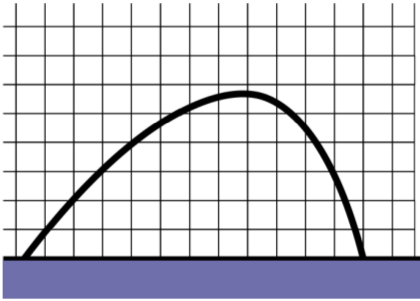
\includegraphics[width=4cm]{1}}
\taskpic{2}{Мальчик Илья играет в хитрый гольф. Ему необходимо попасть в лунку, помеченную флажком, так, чтобы мяч отскочил от очень массивной стенки и не коснулся во время своего движения земли. Стенка приближается к Илье с постоянной скоростью $u$. Илья бьет по мячу так, что начальная вертикальная составляющая скорости мяча равна $v_{\mbox{в}}$. Определите, под каким углом должен изначально полететь мяч, чтобы он попал в лунку и все правила игры были выполнены. В момент удара по мячу расстояние от стенки до Ильи $L_1$, от Ильи до лунки $L_2$.}{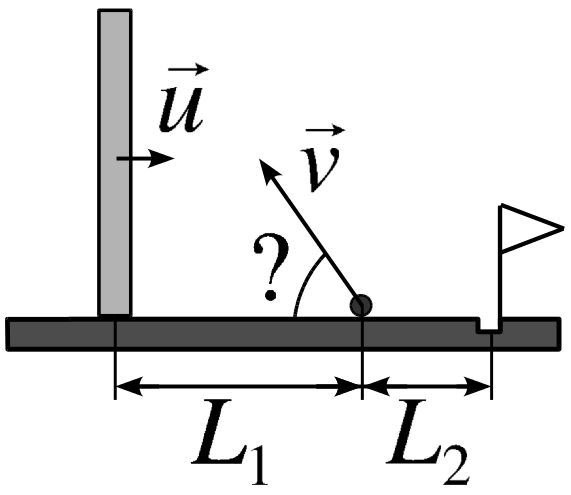
\includegraphics[width=4cm]{2}}
\taskpic{3}{На расстоянии $L=2$~м от кошки сидели мышка и лягушка. Кошка прыгнула так, чтобы поймать их за раз, в этот момент мышь начала убегать, двигаясь по прямой с постоянной скоростью, а лягушка подпрыгнула вертикально с начальной скоростью $U=4$~м/с (см. рис.). Кошка поймала лягушку на лету, а мышку --- при приземлении. Известно, что мышь была поймана через 0{,}8~с после старта. Модуль начальной скорости кошки равен 5~м/с. Найдите скорость мышки и синус угла, под которым прыгнула кошка. Ускорение свободного падения считать равным $g=10$~м/с$^2$. Всех животных считать материальными точками, которые двигаются в одной плоскости. Сопротивлением воздуха пренебречь, пойманная лягушка не влияет на траекторию кошки.}{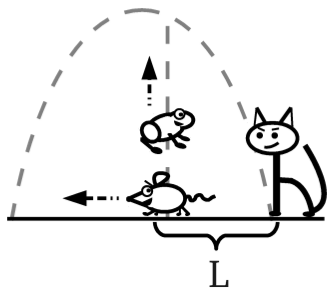
\includegraphics[width=4cm]{3}}
\task{4}{По круговой дорожке радиуса $R=40$~м одновременно стартовали два бегуна. Первый пробегает круг за 20 секунд, а второй --- за 30. Спортсмены бегут по кругу в одну сторону. Через какое время после старта относительная скорость бегунов станет максимальной? Постройте приблизительный график расстояния между бегунами по прямой от времени.}
\taskpic{5}{В солдата, сидящего в окопе, неприятель выстрелил из мортиры (см. рис.). Снаряд летел ровно на него, но до окопа не долетел. С точки зрения солдата снаряд поднимался в течение $t_1$ секунд, а опускался быстрее, за $t_2$ секунд, смотрел он из окопа от уровня земли. Известно, что неприятельские мортиры стреляют под углом $\alpha$ к горизонту, а модуль начальной скорости снаряда равен $V_0$. Найдите, на каком расстоянии от окопа упал снаряд. Сопротивлением воздуха пренебречь, ускорение свободного падения равно $g$.}{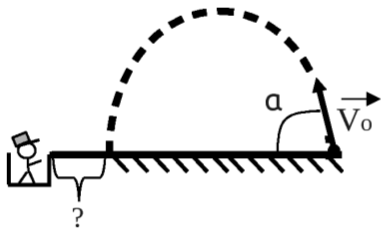
\includegraphics[width=4cm]{5}}
\taskpic{6}{Наклонная плоскость образует угол $\alpha$ с горизонтом. С высоты $H$ на нее падает мячик. Считая удары мячика о плоскость абсолютно упругими, определите расстояние между точками $n$-го и $(n+1)$-го отскока мячика от плоскости.}{
\begin{tikzpicture}[scale=0.7]
\draw (0,2)--(4,0);
\draw (0.5,2.5) node[dot] {} --(0.5,1.75) node[near start,left] {$H$} parabola bend (1,2.2) (1.8,1.1) parabola bend (2.5,1.5) (3.5,0.25);
\draw[dashed] (3.8,0.1)--(2,0.1);
\draw (2.8,0.1) arc (180:153.5:1) node[midway,left] {$\alpha$};
\end{tikzpicture}
}
\taskpic{7}{Тело соскальзывает с гладкой горки с высоты $H$. Отрыв тела от горки происходит на высоте $h$, при этом скорость тела горизонтальна. При каком значении $h$ дальность полета тела будет максимальной?}{
\begin{tikzpicture}[scale=0.7]
\draw (1,3)--(0,3)--(0,0)--(4,0)--(4,1) node[midway,right] {?};
\draw (4,1) parabola (1,3);
\draw[dashed] (1,3.1) parabola[bend at end] (4,1.1) parabola (5.5,0);
\draw[<->] (0.5,0)--(0.5,3) node[midway,right] {$H$};
\end{tikzpicture}
}
\taskpic{8}{Для создания зловещего механизма Мегамозг вскрыл тайное хранилище, содержащее три резистора с сопротивлениями 1~Ом, 4~Ом и 5~Ом. Однако из-за происков врагов надписи на резисторах оказались стерты. Тогда Мегамозг собрал из них верхнюю схему, изображенную на рисунке, и подключил к ней батарейку напряжением 1,2~B. Амперметр показал ток 0,5~А. Затем он собрал нижнюю схему, и, когда он подключил эту схему к батарейке, амперметр сгорел. Однако мастер злодейства не расстроился, ведь теперь он знал, где какое сопротивление. Чему равны сопротивления $R_1$, $R_2$, $R_3$? Амперметр сгорает, если через него течет ток больше 1~А.}{
\begin{tikzpicture}[circuit ee IEC,scale=0.8,thick]
\draw (0,4) to[short,o-] (0.5,4) -- (0.5,4.75) to [resistor={label={$R_1$}}] (2,4.75) to [resistor={label={$R_2$}}] (3.5,4.75) -- (3.5,4) to [ammeter] (4.5,4) node[ocirc] {};
\draw (0.5,4) -- (0.5,3.25) to [resistor={label={$R_3$}}] (3.5,3.25) -- (3.5,4);
\draw (0,1) to[short,o-] (0.5,1) -- (0.5,1.75) to [resistor={label={$R_1$}}] (3.5,1.75) -- (3.5,1) to [ammeter] (4.5,1) node[ocirc] {};
\draw (0.5,1) -- (0.5,0.25) to [resistor={label={$R_2$}}] (2,0.25) to [resistor={label={$R_3$}}] (3.5,0.25) -- (3.5,1);
\end{tikzpicture}
}
\taskpic{9}{Две прямые, пересекающиеся под углом $\alpha$, движутся перпендикулярно самим себе со скоростями $v_1$ и $v_2$.  Определите скорость $v$ точки пересечения прямых.}{
\begin{tikzpicture}
\draw (-2,0.4) -- (1,-0.2);
\draw[->] (-1.6,0.32) -- (-1.45,0.97) node[right,near end] {$\vec{v_2}$};
\draw (-1.8,-0.9) -- (0.8,0.4);
\draw[->] (-1.5,-0.75) -- (-1.2,-1.35) node[right,near end] {$\vec{v_1}$};
\marktheangle{0,0}{0.8,0.4}{1,-0.2}{0.4}{$\alpha$}
\end{tikzpicture}
}
\taskpic{10}{Чиполлино решил сделать светящуюся эмблему своего любимого футбольного клуба <<Зенит>>. Он собрал электрическую схему, как показано на рисунке. Все буквы он составил из неоновых лампочек с одинаковым сопротивлением $R$ (на рисунке толстые черные линии между серыми точками) и соединил их проводами (сопротивление которых пренебрежимо мало, на рисунке тонкие линии). Лампа начинает светиться, если через нее течет сколь угодно малый ток. Нарисуйте, как выглядела светящаяся часть названия клуба, когда Чиполлино подключил напряжение к клеммам 1 и 2. Ответ поясните.}{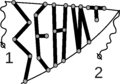
\includegraphics[width=4cm]{10}}
\task{11}{Два одинаковых вольтметра соединили параллельно, третий вольтметр подключили к этой комбинации последовательно, и к концам получившейся цепи присоединили идеальную батарейку. При этом вольтметры показывают 4~В, 4~В и 5~В. Какое напряжение у батарейки? Могут ли быть одинаковыми все три вольтметра? Что покажут эти же приборы, если их все соединить последовательно и подключить к той же батарейке? Показания приборов считайте точными.}
\task{12}{Рядом стоят две пушки, из которых можно стрелять теннисными мячиками под любым углом к горизонту с начальной скоростью $v=20$~м/с. Из пушек одновременно стреляют в бубен, находящийся на расстоянии $L=20$~м по горизонтали, однако удары мячиков о бубен происходят не одновременно. Найдите время между ударами. Расстоянием между пушками, размером бубна, а также сопротивлением воздуха пренебречь. Ускорение свободного падения $g=10$~м/с$^2$.}
\taskpic{13}{Два одинаковых бруса скрепили за середины торцов одинаковыми нерастяжимыми нитями и положили на угол стола (см. рис.). Торцы выступают за края столешницы так, что нити не касаются стола. Коэффициент трения о вертикальную поверхность стола в 3~раза больше, чем о горизонтальную. Известно, что если поставить систему с начальным углом нити к горизонтали $\alpha < 45^\circ$ (см. рис.), то бруски начнут двигаться, тогда как если в начальный момент $\alpha \geqslant 45^\circ$, то система остается неподвижной. Найдите коэффициент трения о горизонтальную поверхность.}{
\begin{tikzpicture}[scale=0.35]
\draw (0,0)--(5,0)--(5,-5);
\draw (1.5,4)--(8,4)--(8,-3.5);
\draw (5,0)--(8,4);
\filldraw[fill=gray] (1,0) -- (3,0) -- (6,4) -- (6,6) -- (4,6) -- (1,2) -- cycle;
\draw (1,2) -- (3,2) -- (3,0);
\draw (3,2) -- (6,6);
\filldraw[fill=gray] (5,-4) -- (7,-4) -- (10,0) -- (10,2) -- (8,2) -- (5,-2) -- cycle;
\draw (5,-2) -- (7,-2) -- (7,-4);
\draw (7,-2) -- (10,2);
\draw (2,1) node[dot] {} --(6,-3) node[dot] {};
\draw[dashed] (5,5) node[dot] {}--(9,1) node[dot] {};
\draw[dashed] (2,-3)--(6,-3);
\draw (4,-3) arc (180:135:2) node[midway,left] {$\alpha$};
\end{tikzpicture}
}
\taskpic{14}{B системе, изображенной на рисунке, пружины имеют жесткости $k_1=100$~Н/м и $k_2=200$ Н/м. К нижнему блоку подвешивают груз массой $M=8$~кг. Система приходит в равновесие. На сколько сместился нижний блок? Пружины, нити и блоки невесомы. Нити нерастяжимы. Ускорение свободного падения $g=10$~м/c$^2$.}{
\begin{tikzpicture}[scale=0.8]
\draw[interface] (0,5)--(2.5,5);
\draw (0.5,5)--(0.5,4.5);
\draw[spring] (0.5,4.5)--(0.5,3.5) node[midway,left] {$k_1$};
\draw (0.5,3.5)--(0.5,3);
\draw (1,3) circle [radius=0.5];
\draw (1.5,3)--(1.5,5);
\draw (1,3)--(1,1.5);
\draw (1.5,1.5) circle [radius=0.5];
\draw (2,1.5)--(2,3.5);
\draw[spring] (2,4.5)--(2,3.5) node[midway,right] {$k_2$};
\draw (2,4.5)--(2,5);
\draw (1.5,1.5)--(1.5,0.5);
\filldraw[fill=gray] (1,0.5) rectangle (2,0) node[right] {$M$};
\end{tikzpicture}
}
\taskpic{15}{На гладкой наклонной плоскости, составляющей с горизонтом угол $\alpha=30^\circ$, расположен массивный клин (см. рис.). На верхней горизонтальной поверхности клина лежит маленькая легкая шайба. Клин отпускают, и он начинает свободно соскальзывать вниз.
\begin{compactenum}
\item Определите величину и направление ускорения движения шайбы относительно наклонной плоскости.
\item Как выглядит движение шайбы в системе отсчета, связанной с клином?
\end{compactenum}
Масса шайбы много меньше массы клина. Трением пренебречь.}{
\begin{tikzpicture}[scale=1.2]
\draw (0,1.5)--(3,0);
\draw[dashed] (0.5,0.5)--(2,0.5);
\filldraw[fill=gray] (0.5,1.27)--(2.5,0.27)--(2.5,1.27)--cycle;
\filldraw[fill=black] (1.6,1.28) rectangle (1.8,1.38);
\draw[thick] (1.5,0.5) arc (180:153.5:0.5) node[midway,left] {$\alpha$};
\end{tikzpicture}
}
\taskpic{16}{Три одинаковых бревна, имеющих форму цилиндра, сложены так, как показано на рисунке. Какие минимальные коэффициенты трения бревен друг по другу и бревен по земле необходимы для того, чтобы система оставалась в покое?}{
\begin{tikzpicture}
\draw[interface] (3,0)--(0,0);
\draw (1,0.5) circle [radius=0.5];
\draw (2,0.5) circle [radius=0.5];
\draw (1.5,1.366) circle [radius=0.5];
\end{tikzpicture}
}
\task{17}{Вася любит принимать ванну и знает, что для него комфортная температура воды 35$^\circ$C. К сожалению, у него на несколько дней отключили холодную воду. Вася померил температуру горячей воды, вытекающей из крана (60$^\circ$C), и заметил, что можно комфортно сидеть в набирающейся ванне, если каждые 7~секунд бросать в нее кубик льда из морозильника. На следующий день оказалось, что ледяные кубики приходится бросать каждые 5~секунд, хотя поток воды из крана такой же. На сколько изменилась температура воды в кране? Тепловыми потерями пренебречь, вода быстро перемешивается и кубики тают быстро.}
\taskpic[6cm]{18}{На примусе, расходующем $\mu = 0{,}1$~кг бензина в час, стоит котелок, в котором находится $m = 1$~кг воды. График зависимости тепловой мощности $P$, выделяемой в окружающую среду, от времени приведен на рисунке. Постройте график зависимости температуры воды в котелке от времени. Теплоемкость котелка $C = 800$~Дж/$^\circ$C, удельная теплоемкость воды $c_0 = 4200$~Дж/(кг$\cdot^\circ$C). Удельная теплота сгорания бензина $q = 43$~МДж/кг. Начальная температура воды $T=20^\circ$C. Принять, что в любой момент времени температура котелка и воды совпадают.}{
\begin{tikzpicture}
\begin{axis}[
    width=6cm,
    xmax=10.5,
    ymax=1000,
    xtick={0,2,...,10},
    ytick={0,200,...,1000},
    grid=both,
    minor tick num=3,
    major grid style=thick,
    minor grid style=thin,
    axis lines=middle,
    axis line style={->},
    xlabel={$t$, мин},
    ylabel={$P$, Вт},
    /pgf/number format/1000 sep={\,},
]
\addplot[thick,domain=0:10] {1200 * (1 - exp(-x/7))};
\end{axis}
\end{tikzpicture}
}
\task{19}{В морозильной камере, потребляющей из сети мощность 100~Вт, находится 20~кг воды при температуре 0$^\circ$C. За 1~час вся вода замерзла. Какое количество теплоты за это время выделилось в окружающую среду? Теплота плавления льда 330~кДж/кг. Считать, что в процессе замерзания температура льда остается постоянной, равной 0$^\circ$C.}
\taskpic[5cm]{20}{Любознательный школьник разобрал нагревательный прибор. Оказалось, что схема прибора очень проста (см. рисунок). Школьник вынул все резисторы из схемы и обнаружил, что их сопротивления составляют $R_1=1$~Ом, $R_2=1$~Ом, $R_3=2$~Ом, $R_4=3$~Ом, $R_5=5$~Ом. Но он забыл, какой резистор на каком месте располагается в схеме. Помогите ему собрать прибор по старой схеме таким образом, чтобы его мощность была максимальной. Нагреватель работает от постоянного напряжения.}{
\begin{tikzpicture}[circuit ee IEC,thick,scale=0.8]
\draw (0,0) to[short,o-] (0.5,0) -- (0.5,0.75) to [R] (2,0.75) to [R] (3.5,0.75) to [R] (5,0.75) -- (5,0) to[short,-o] (5.5,0);
\draw (0.5,0) -- (0.5,-0.75) to [R] (2.75,-0.75) to [R] (5,-0.75) -- (5,0);
\end{tikzpicture}
}
\task{21}{Тело роняют над плитой на высоте $h$ от нее. Плита движется вертикально вверх со скоростью $u$. Определите время между двумя последовательными ударами тела о плиту. Удары абсолютно упругие.}
\task{22}{Утюг устроен следующим образом: его нагреватель выключается, если температура утюга становится больше некоторой температуры $t_2$, и включается, как только его температура падает ниже $t_1$ (эти температуры неизвестны). Если включенный утюг стоит с открытой металлической поверхностью, его нагреватель работает в среднем $k=1/4$ всего времени. При этом мощность теплоотдачи можно считать постоянной. Если утюгом начинают гладить, то промежуток времени между последовательными моментами включения нагревателя становится в $n=4/3$ раза меньше. В этом случае мощность теплоотдачи также остается постоянной. Какую часть времени он работает в среднем во втором случае?}
\taskpic{23}{Школьница Василиса проводит опыты с пружиной. Сначала Василиса обнаружила, что длина пружины в нерастянутом состоянии составляет 10 см, а груз массой $m$~г, подвешенный к пружине, дополнительно растягивает ее на $0{,}01m$~см. Затем Василиса подвесила пружину с грузом над сосудом в форме прямоугольного параллелепипеда, как показано на рисунке, и стала наливать в сосуд воду. Груз имеет форму куба длиной ребра 10~см, его плотность равна плотности воды. В начале опыта расстояние от нижней грани груза до дна сосуда составляет 30~см. Площадь основания сосуда составляет 1000~см$^2$. Нижняя грань куба во время опыта сохраняла горизонтальное положение. Постройте график зависимости длины пружины $l$ от объема воды $V$, налитой в сосуд. При каких значениях объема $V$ груз находился в воздухе? был частично погружен в воду? был полностью погружен в воду?}{
\begin{tikzpicture}[scale=0.5]
\draw[interface] (1,8)--(3,8);
\draw (2,8) -- (2,7);
\draw[spring] (2,7) -- (2,5);
\draw (2,5) -- (2,4);
\draw (1.5,4) rectangle (2.5,3);
\draw (0,6) -- (0,0) -- (4,0) -- (4,6);
\end{tikzpicture}
}
\task{24}{Фонтан в Женеве бьет на высоту $h$. Расход воды составляет $P$ кг за 1 секунду. Найдите площадь сечения сопла фонтана. Ускорение свободного падения равно $g$, плотность жидкости $\rho$. Пренебречь сопротивлением воздуха, поверхностным натяжением и вязкостью жидкости.}
\taskpic{25}{На горизонтальный скользкий цилиндр аккуратно, без зазоров намотали широкую ленту. На оба конца ленты подвесили одинаковые грузики массы $m$. Давление ленты на цилиндр при этом оказалось равно $P$. Найдите диаметр окружности цилиндра. Ширина ленты $l$, ускорение свободного падения $g$. Массой ленты по сравнению с массой грузов пренебречь, трение ленты о саму себя и о цилиндр отсутствует. Ширина ленты много меньше диаметра окружности цилиндра.}{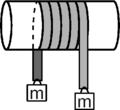
\includegraphics[width=3cm]{25}}
\taskpic{26}{Шар массы $m_1$ налетает со скоростью $v$ на покоящийся шар массы $m_2$. Между ними происходит центральный, абсолютно упругий удар. Какая часть кинетической энергии первого шара перейдет ко второму? Постройте график зависимости доли переданной энергии от массы $m_2$.}{
\begin{tikzpicture}
\draw (0,0) circle [radius=0.3] node[below=0.3cm,anchor=north] {$m_1$};
\draw[->] (0.3,0) -- (1.3,0) node[midway,anchor=north] {$\vec{v}$};
\draw (2.5,0) circle [radius=0.5] node[below=0.5cm,anchor=north] {$m_2$};
\end{tikzpicture}
}
\end{document}
